\begin{frame}{Multilevel Monte Carlo Implementation}

 \begin{center}
    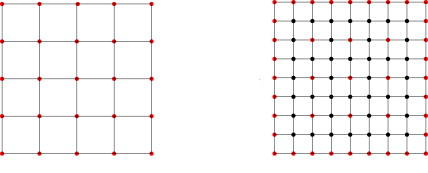
\includegraphics[height=3cm]{presentation_graphics/fine_grid_vs_coarse_grid.png}
\end{center}   

{\footnotesize
\begin{columns}[T] 
  \begin{column}{0.48\textwidth}
    \centering
    \textbf{Stochastic Heat Equation (SHE)}
    \begin{align*}
        U_j^{n+1} &= U_j^n + \lambda (U_{j+1}^n - 2U_{j}^n + U_{j-1}^n) + \Delta W_j^n 
        \vphantom{\frac{F_{j+1}^{\,n}}{2\Delta x}}
        \\
        U_j^0 &= 0, \ U_0^n = U_J^n = 0 \\
        \hat{P} &= (U^n,U^n)_{\Delta x} \quad \hat{P} = \left(U, \phi_n\right)_{\Delta x}^2
    \end{align*}
  \end{column}
  %
  \begin{column}{0.48\textwidth}
    \centering
    \textbf{Dean-Kawasaki (DK) Equation}
    \begin{align*}
        \rho_j^{\,n+1} &= \rho_j^{\,n} + \tfrac{\lambda}{2}\,\bigl(\rho_{j+1}^{\,n}-2\rho_j^{\,n}+\rho_{j-1}^{\,n}\bigr)
        + \tfrac{1}{\sqrt{N_p}}\,
        \frac{F_{j+1}^{\,n}-F_{j-1}^{\,n}}{2\Delta x} \\
        \rho_j^0 &= \rho_0(x_j), \quad \rho_0^n = \rho_J^n, \\
        P &= N_p \left( \big(\rho^n - \bar\rho^n,\ 
        \sin(\Delta x)\big)_{\Delta x} \right)^{\!2}
    \end{align*}
  \end{column}
\end{columns}
}

    \begin{textblock*}{9cm}(4.8cm,4.5cm)
        \scalebox{0.7}{
            Coarse Mesh
        }
    \end{textblock*}
    \begin{textblock*}{9cm}(9.65cm,4.5cm)
        \scalebox{0.7}{
            Fine Mesh
        }
    \end{textblock*}
\end{frame}
